\section{Tubular Inputs and Outputs}

\valkyrie{What do you guys think about trying to merge this with the example objects section?  It would cut down the text a lot, but it might seem weird to just shunt those in here.}

Once objects have been designed and fabricated, the major flexibility for prototyping with pipes stems from the media inserted in them.  The five types of media--gas, liquid, solid, particulate, and threadable--give rise to unique possibilities in output (visual, aural, tactile/haptic, olfactory/gustatory) as well as input (touch/pressure and others).

\tovi{There's lots of great ideas an examples in the inputs and outputs section, but the orgnization and coorespondence to the table is a little hard to follow. }

By crossing pipe types, topologies, and inserted media, we create a space of possible inputs and outputs that can be pipe-mediated.  We offer a table (see Figure \ref{fig:designspace}) containing these possibilities, referencing previous work on input/output techniques where appropriate, noting that many of these techniques have not been attempted using digital fabrication.  We suggest new points in the design space that have been unexplored or not yet explored with digital fabrication.

\begin{figure*}[t]
\centering
    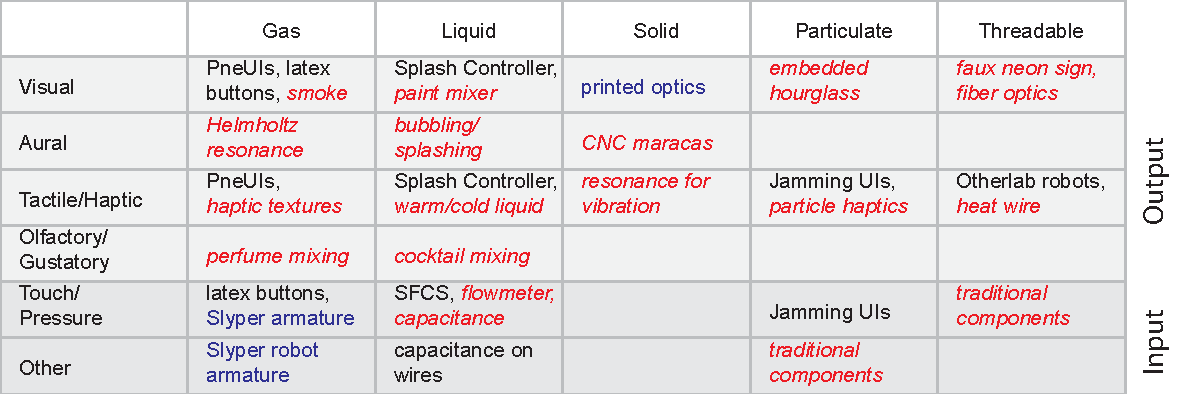
\includegraphics[width=\textwidth]{figures/designspace.pdf}
\caption{The design space of pipe-based interactions.  Existing systems are written in regular font.  Those created with fabrication are in {\color{blue}blue}. In \emph{{\color{red}red italic}} are unexplored interactions creatable with custom-fabricated pipes. \tovi{Im not sure how well this table will work. Division between input and output should be more prominent.} \valkyrie{one possibility is making the table larger and adding some short descriptions.  we could throw out a lot of words from the paper that way}}
\label{fig:designspace}
\end{figure*}

\subsection{Outputs}

We describe potential pipe-based outputs organized by the five senses: visual, aural, haptic, and olfactory/gustatory.  In addition to outputs we mention explicitly, any outputs possible using traditional electronic components are possible as described above.

\begin{figure}[h]
\centering
    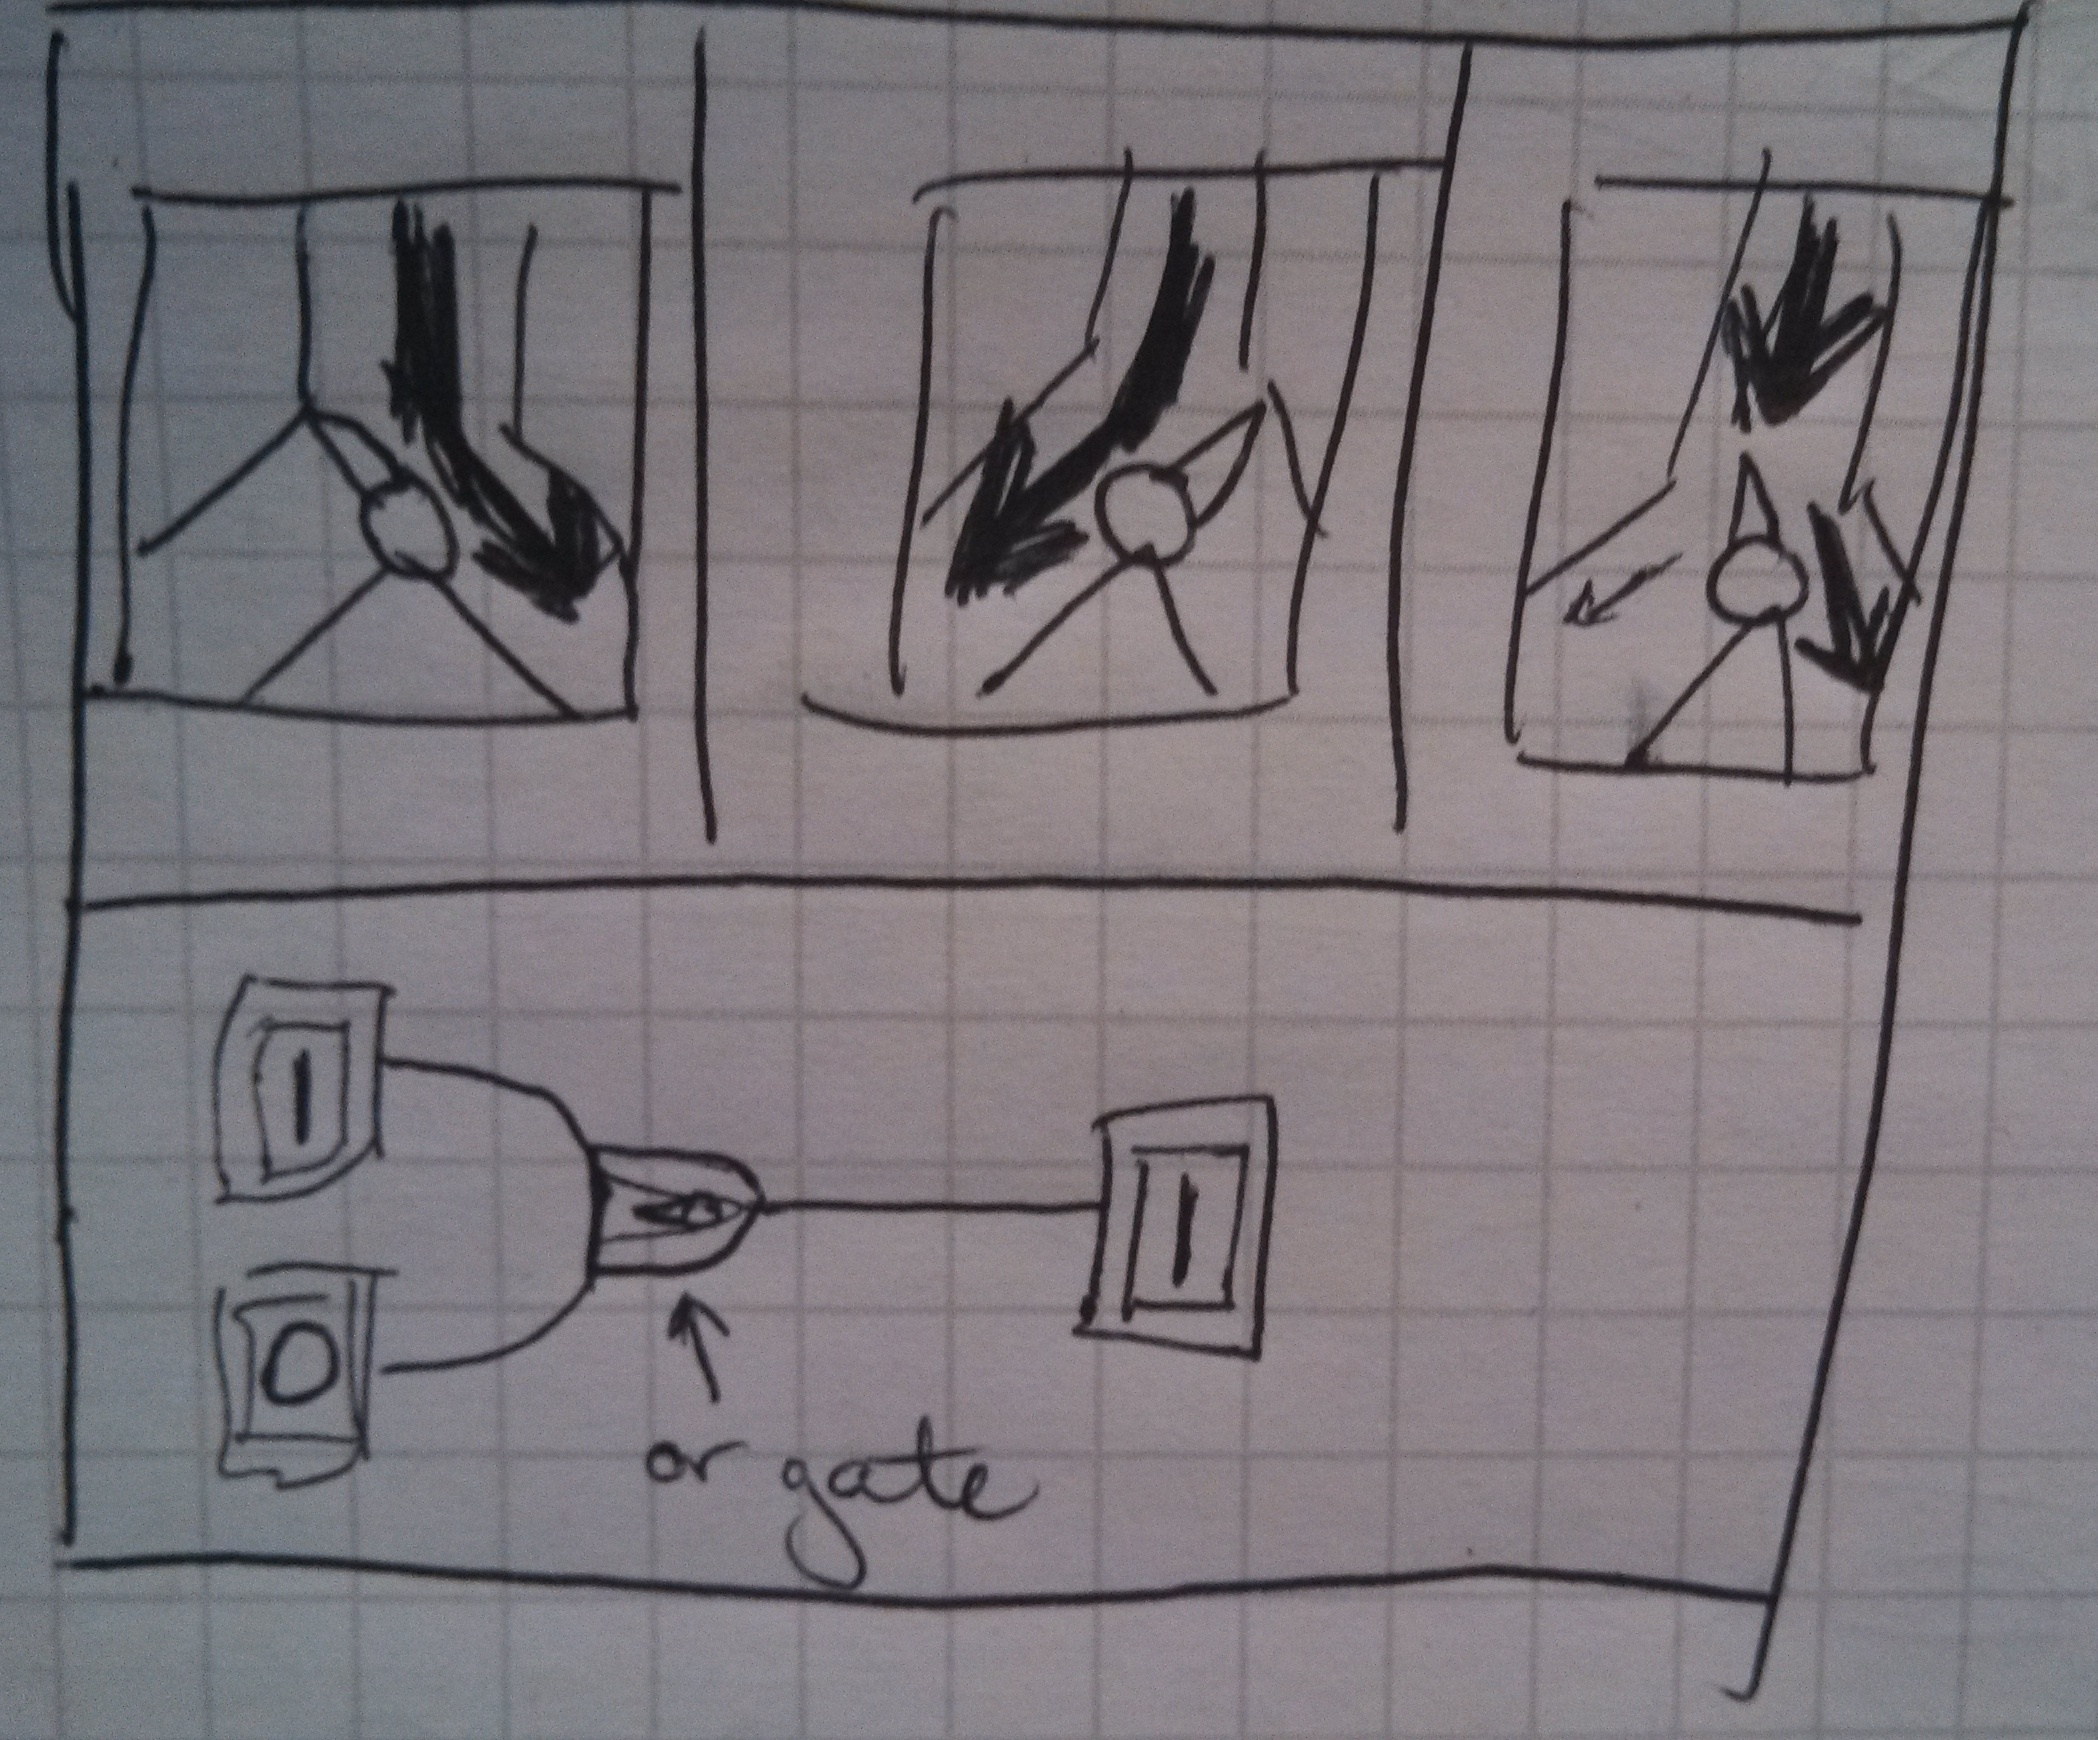
\includegraphics[width=3.4in]{figures/placeholder/direct.jpg}
\caption{By attaching a servo to a gate structure, it is possible to direct fluid through that pipe.  The gate not only has binary positions (a) and (b), but can direct fractional flow, as well (c).  This could be used to create logic gates, as in (d).  These could be used, for example, in science exhibits.}
\label{fig:direct}
\end{figure}

\emph{Visual} outputs can be mediated by gases, liquids, solid, particulates, or threadables.  Pneumatic actuation (as in \cite{Yao-pneui} or \cite{Harrison-buttons}) provides output, but gases carrying smoke (as in \cite{Sodhi-aireal} demo) also offers visual feedback.  Splitting and mixing of colored liquids can be used as a display tactic; additionally mechanical motion can be fluid-mediated.  Liquids can also be mixed in specific concentrations by servo-controlled gate structures as in Figure \ref{fig:direct}.  Printed optics \cite{Willis-printedoptics} explored visual output at the ends of pipes, and   EL wire can be threaded through custom paths to create neon signs, as in Figure \ref{fig:neon}.

\emph{Aural} outputs can be created with gases.  Helmholz resonance can be leveraged to create computer-controllable sound chambers, as in Zoran's flute \cite{Zoran-flute}.  All that is necessary for this is an enclosed chamber with a pipe connected to it via a narrow neck-point (see Figure \ref{fig:ocarina}).  Passive sound amplification and sound redirection are also possible using pipes.

\begin{figure}[h]
\centering
    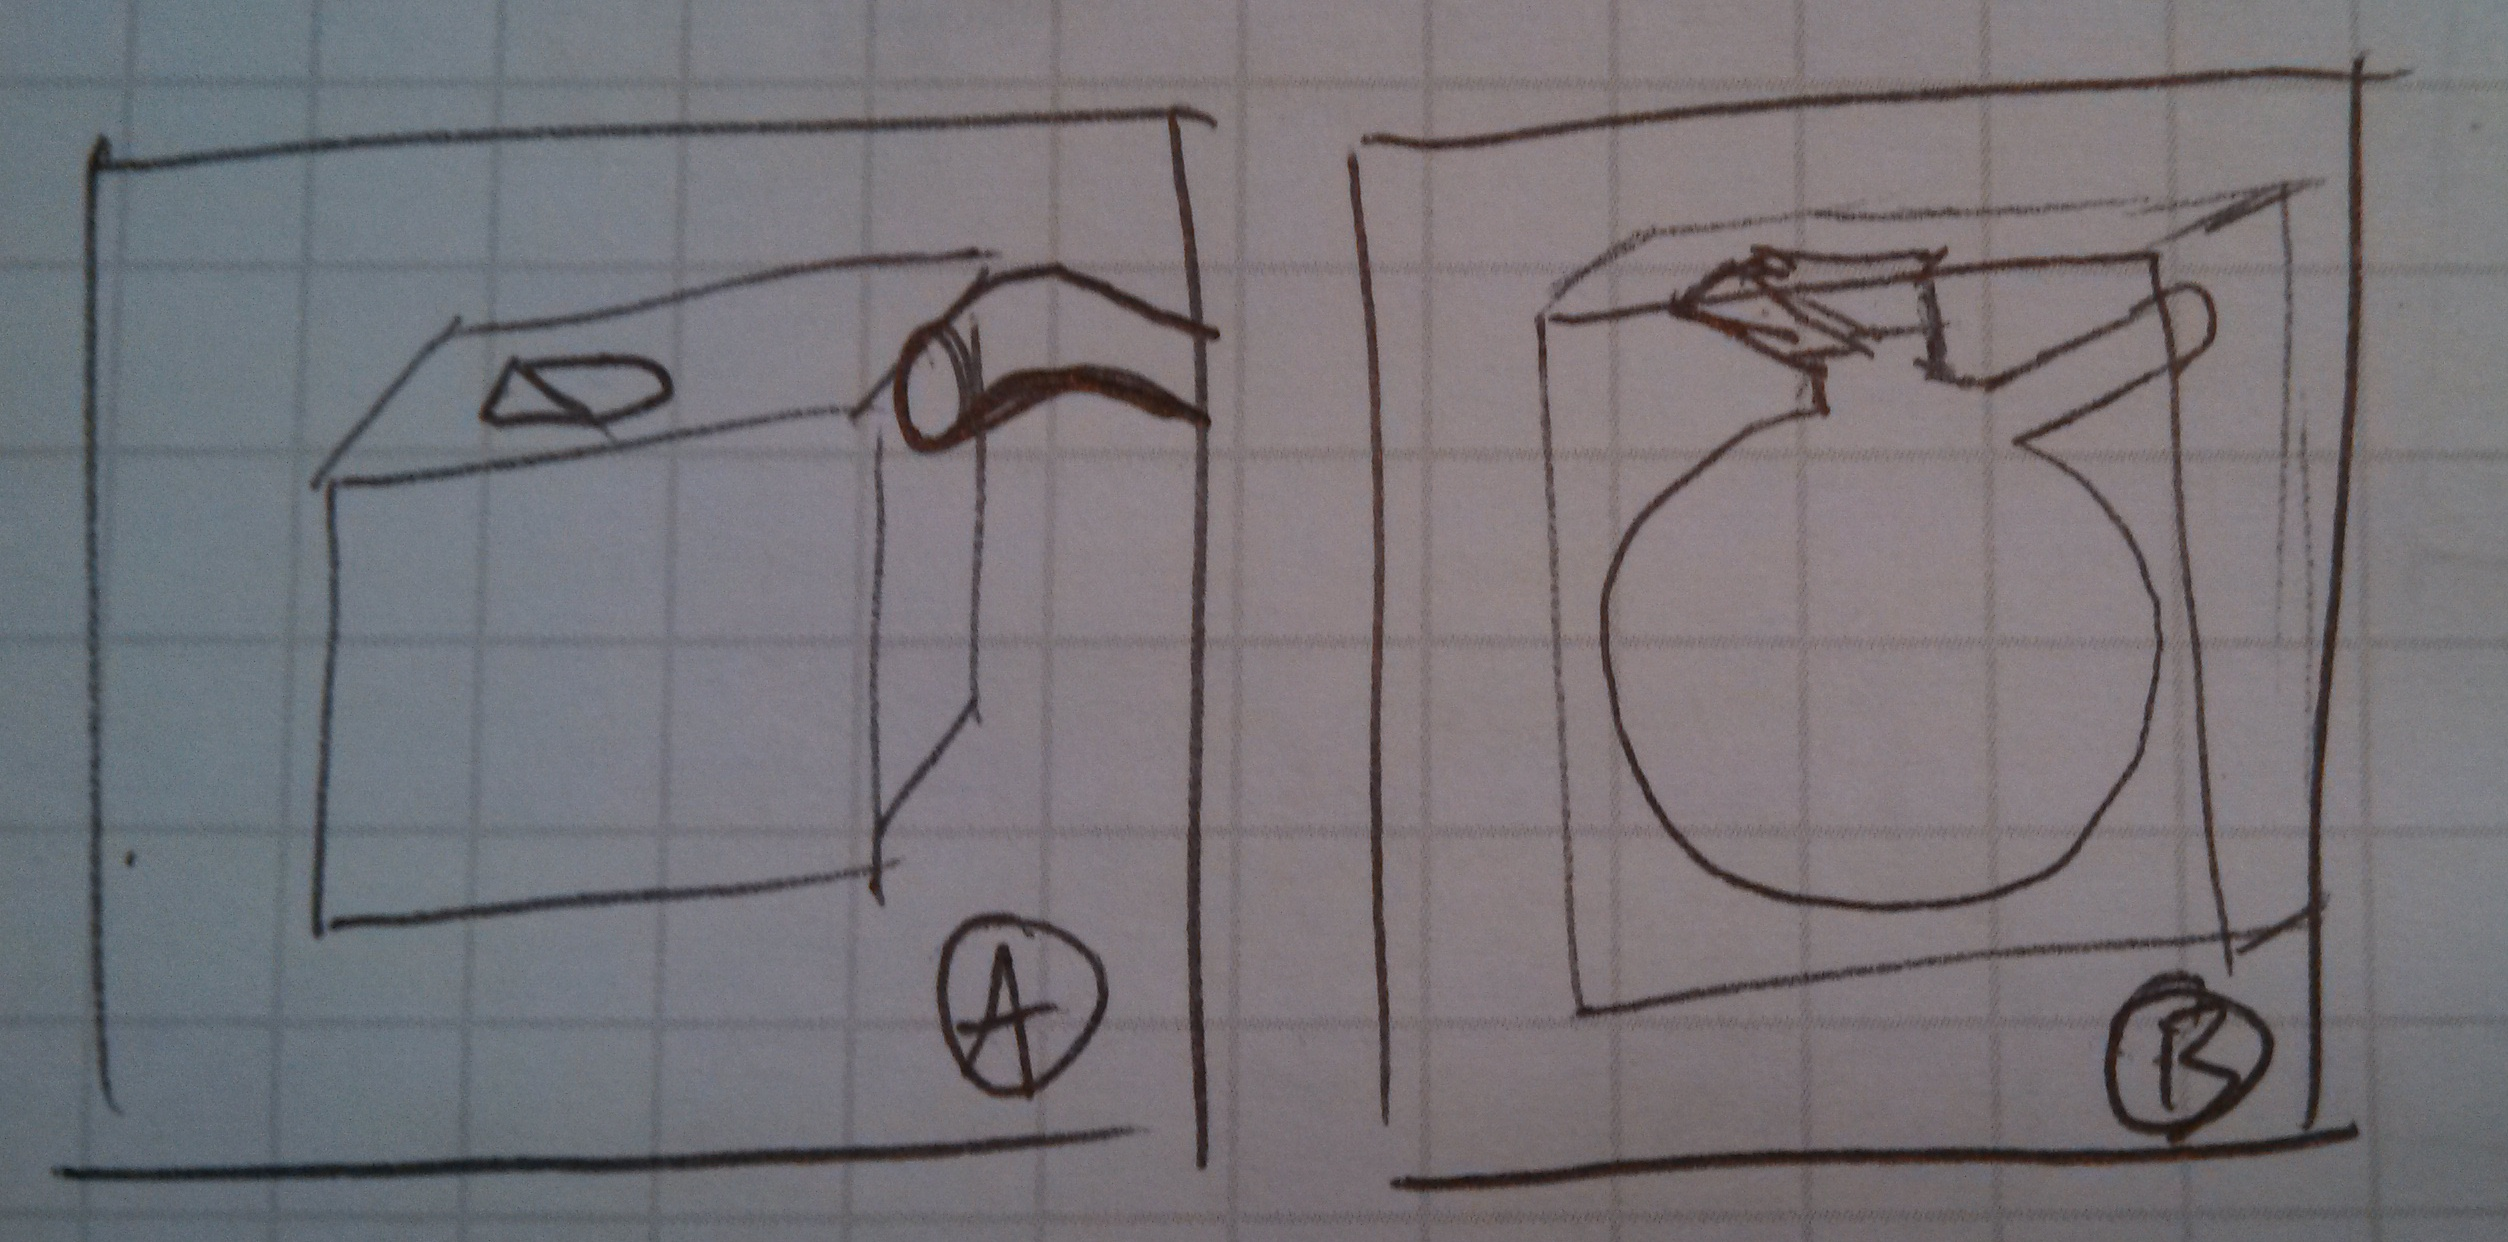
\includegraphics[width=3.4in]{figures/placeholder/helmholz.jpg}
\caption{This box (a) contains an enclosed Helmholz resonator, seen in the cutaway view (b).  This resonator creates a sound when air is blown through the pipe at the top, because air compresses at the small neck joint between the chamber and the pipe.  \valkyrie{need to get a test print of this that actually works}}
\label{fig:ocarina}
\end{figure}

\emph{Haptic} outputs are possible through compressible and incompressible fluids.  Fluids can actuate particulates and create programmable pliability \cite{Follmer-jamming}.  Additionally, use of semi-closed pipes with rubberlike material as the caps allows for gases to actuate surface features (see Figure \ref{fig:breathe}).  Free-air haptic feedback \cite{Sodhi-aireal} and volumetric interactions \cite{Iwata-volflex} can be pipe-mediated.

\emph{Olfactory} and \emph{gustatory} outputs can be created through the mixing and splitting of pipes carrying scented or flavored fluids, respectively.

\subsection{Inputs}

Pipes create opportunities for many types of input sensing across the surface of printed devices.  We describe sensing touch, pressure, grasp, flexing, tapping, and manipulation of traditional electronic components.  There are likely more input sensing techniques, both existing and on the horizon, that are compatible with the use of pipes.

\emph{Touch} sensing can be enabled through pipes filled with conductive media.  Traditional wires (threadable) may be used, but conductive paint (liquid) may be more flexible.  Using conductive paint and Swept Frequency Capacitive Sensing (SFCS \cite{Sato-touche}), an interior star pipe topology can enable single-wire touch- and grasp-sensing at any set of points on a printed object's surface (see Figure \cite{fig:toys}).  Simple capacitance measurements are possible using the same media, and custom-designed sensors like those created in Savage, et al.,'s Midas system are also possible \cite{Savage-midas}.

\emph{Pressure} can be sensed in multiple ways.  Slyper, et al.,'s primitives can be attached as the terminus of any semi-closed pipe; the user can manipulate the printed endpoint and the system can sense air pressure changes \cite{Slyper-pressure}.  Pressure can also be sensed via capacitance.

\emph{Grasp} sensing can be enabled using Wimmer's FlyEye techniques \cite{Wimmer-flyeye} or those described in Jamming User Interfaces \cite{Follmer-jamming}.  The optical links necessary for sensing can be created either via clear solid cores as in \cite{Willis-printedoptics} or via fiber optic cables threaded through hollow pipes (see Figure \ref{fig:pens}).

Some 3D printers can fabricate rubber-like materials.  Similar to Slyper, et al., in \cite{Slyper-shape}, we can sense \emph{flexing} and \emph{bending} of prints made on these machines: the ability to 3D print devices to sensing bending and flexing significantly cuts molding and assembly time.

\emph{Tapping} is another input possibility.  Due to differential sound conductivity in different printed materials, pipes of a greater conducting material can be embedded in a model of a lesser conducting material.  A microphone or piezo placed at the system-side of these sound-conducting pipes can determine where the model was tapped and how it was tapped.  Active acoustic sensing as described in Touch \& Activate \cite{Ono-touchandactivate} is also possible; this technique would allow for particular areas of interest (connected to sound-conducting pipes) to be touch sensitive, while other areas (made of non-conducting material) are not sensed.

Sensing via traditional electronic components (e.g., potentiometers, alcohol gas sensors) can be accomplished by conductive inserted media.  Components can be recessed into a print's surface, with their leads implanted into open pipes.  By inserting liquid copper paint instead of threading traditional wires, all components in a model can share a ground line, and the paint's drying process obviates the use of solder or glue to affix the components in place (see Figure \ref{fig:radio}).

\subsection{Fabrication Techniques}

The physical fabrication process used by different machines gives rise to differing design guidelines.  The two machines we used to create our example objects were the Objet Connex 260 and the Makerbot Replicator 2.

The Objet is an inkjet-based 3D printer which jets drops of polymer in very fine layers, curing each layer with an ultraviolet lamp.  It offers a wide range of material types, including clear/opaque, flexible/hard, and black/white.  Additionally, it permits the mixing of two different materials in a single print: a mixed material could include 70\% flexible and 30\% hard, for example, to be firm but somewhat flexible.  The flexible materials can be inflated when they are thin: they elongate 200\% before breaking.  We have found $.05$inches to be a good thickness for inflatable materials.  Although this machine has many extraordinary capabilities, it unfortunately cannot print overhangs of greater than $14^{\circ}$ without support material.  The support structure used by this machine is a loose matrix of material that can be removed by hand from the surface or blasted out with a water jet from the interior.  The support is also soluble in lye.

The Makerbot Replicator 2 is a fused-deposition modeling (FDM) printer, in which we use exclusively Polylactic Acid (PLA) bioplastics.  More material properties are being explored in PLA: there are now transparent and flexible materials.  They cannot be blended like those in the Objet.  The Makerbot has a fairly coarse resolution compared to the Objet, however it permits overhangs up to $45^{\circ}$ without support and also allows bridging (short spans of material that bridge the gap between two structures with no support underneath).  Due to the FDM process it can even recover from greater overhangs and longer bridges, as the material builds up and can reorganize into a structure \valkyrie{how do I say this?  do I need a photo?  print recovery is pretty awesome-looking.}.  The support used by the Makerbot is made of the same material as the model itself, just printed in a different pattern and attached over as small a surface area as possible to ease removal.  Support inside of a pipe may require pliers, or be infeasible to remove dependent upon geometry.

Assembly is easiest on both machines when the model does not require support material.  Models can be ``cut up'' into assembleable pieces to evade support requirements or ease material removal.  We believe that an automatic tool for this task would be highly beneficial, however it is outside the scope of this work.